\chapter{System Description}
\setlength{\parindent}{15pt}
\label{ch:syst_desc}

% what is this chapter about - Joel
In this chapter, the system will be considered on a deeper level of detail; the system is broken down into subsystems. In \autoref{sec:subs_inte} these subsystems are defined and the elements they are comprised of, are identified. \autoref{sec:inter} deals with the interrelations between the individual subsystems on design level; this is illustrated by means of a $N^2$ chart. \autoref{sec:subs_requ} states the subsystem requirements and constraints, which create the design space in which the designing has to be performed. \autoref{sec:mass_cost_powe_brea} describe the mass, cost and power budgets; the total budgets are broken down and divided among the different subsystems. Since there is still an aspect of uncertainty at this stage of the design process, contingencies are incorporated in the budgets. These contingencies are justified in \autoref{sec:budg_cont}.

\section{Subsystem Definition}
\label{sec:subs_inte}

%%% Subsystems introduction (5 sections) - Piotr
Subsystems are groups of elements within a system, which have a physical or functional commonality. Systems are divided into these groups in order to have a better overview of either the functionality or the design process, making it more approachable. The latter is especially valuable when working on larger projects such as the UAV system at hand. Therefore, it is sensible to split this system into subsystems as well. The subsystems and the responsible engineering departments are explained below, whilst the elements contained within each subsystem are listed in \autoref{tab:elem_subs}.\\

%explain structure of this section - relation, department allocation

%%% how we found subsystems - whiteboard image - Joel
\noindent \textbf{Structure: fuselage, wing, and tail:} Primarily, the main structural subsystems are addressed; the fuselage, the wing and the tail section. The fuselage is regarded as the main frame work; the attachments with the wing and the tail are regarded as 'fuselage' responsibility.

The first allocated department is the aerodynamics, due to the influence these subsystems have on the aerodynamic characteristics of the UAV.  Furthermore, the structures department is involved, because the fuselage, wing and tail form the main framework and thus they must provide the structural integrity to the UAV.\\

\noindent \textbf{Propulsion:} Next to the main structural aspect, the propulsion is regarded as an individual subsystem; both physically and functionally. Physically it is developed and assembled separately, due to its external mounting. Furthermore, there are several top level requirement related to the VTOL capability and the high speed performance that are specific to the propulsion unit. Thus, functionally speaking, the propulsion system is regarded a separate subsystem as well.

The propulsion subsystem includes the pylon, which forms the interface with the wing. This is regarded as a structural aspect. That is why the structural department is consulted in the development of the propulsion subsystem. Furthermore, there are several factors related to aerodynamics as well; not only the shape of the pylon, but also the feathered or folded propeller has strong affinity with the aerodynamics department. The propeller design itself is treated by the power \& propulsion department. Finally, the control \& stability department will be involved, since stability and control is significantly related to the propulsion system, especially in vertical take-off and hovering.\\

\noindent \textbf{Power:} The power management and distribution on board of the UAV is also selected to be its own subsystem. The main reason is that the only power source for all the other subsystems is electrical, making the power subsystem an essential and significant element of the system. Due to its great importance, it requires a dedicated development section.

The power \& propulsion department is the only department that will be involved in the design of the power subsystem.\\

\noindent \textbf{Avionics and ground station:} Aviation related electronics that enable autonomous and supervised control lead up to the avionics and ground station subsystems. These two systems are composed of enough elements to be individual subsystems. \\ \indent The responsible department will be the Command \& Data Handling, since this department specialises in the data collection and processing within the UAS.\\

\noindent \textbf{Payload bay:} Although the payload bay was considered part of the fuselage section at first, later it was given a subsystem status. The subsystem needs to have a broad operational flexibility; there are several mission related requirement that result in a more complicated design. The resulting increased effort required for the design is so substantial, that it justifies the choice of making the payload bay a separate subsystem.\\ \indent Logically, the structures department is one of the involved parties; both for the implementation in the fuselage and for the payload hatches which enable drop-off mission. Besides structures, Command \& Data Handling will be involved to design the interface between the payload and the communication system. Also the interface with the power subsystem has to be considered; in some mission settings, the payload bay will be used to extent the battery capacity. That is why there is a connection with the Power \& Propulsion department.

\begin{table}[h]
\centering
\caption{Elements Incorporated within Subsystems}
\label{tab:elem_subs}
\begin{tabular}{lll}
\toprule
\textbf{Subsystems}     & \multicolumn{2}{c}{\textbf{Elements}}                               \\\midrule
\textbf{Fuselage}       & Internal layout            & Attachment fuselage - wing   \\
\textbf{}               & Structure                  & Attachment fuselage - tail   \\
\textbf{}               & Payload bay integration    & Battery mounting              \\\hdashline
\textbf{Wing}           & Control surface            & Structure                     \\
\textbf{}               & Actuator                   & Landing gear                  \\
\textbf{}               & High lift device           & Attachment wing - propulsion unit \\
                        & Wingtip devices            &                               \\\hdashline
\textbf{Tail}           & Structure                  & Actuator                      \\
\textbf{}               & Control surface            &                               \\\hdashline
\textbf{Propulsion unit}     & Motor                      & Storing/feathering mode       \\
\textbf{}               & Propellers                 & Motor controller              \\
\textbf{}               & Tilting mechanism          & Pylon structure               \\\hdashline
\textbf{Power unit}          & Battery unit               & Electrical elements           \\
\textbf{}               & Cable hardness             &                               \\\hdashline
\textbf{Avionics}       & Flight Control Module                        & Communication system          \\
\textbf{}               & Sensors                    & Autopilot                     \\
\textbf{}               & Navigation system          & Safety system                 \\\hdashline
\textbf{Payload}        & Payload mounting           & Data transmission             \\
\textbf{}               & Payload hatch              & Power connector               \\\hdashline
\textbf{Ground station} & CPU                        & Controller (input device)            \\
\textbf{}               & Display (visual interface) & Casing                        \\
                        & Communication system       & Power supply                  \\
                        & Maintenance unit           & Antenna tracking system       \\\bottomrule
\end{tabular}
\end{table}

\section{Subsystem Interrelations}
\label{sec:inter}

%%%% Piotr
Although the definition of the subsystems gives a general overview of the design process, it is not sufficient to be useful during the design process itself. To solve this problem, it is necessary to define the relations between the subsystems in the form of an $N^{2}$ chart. This makes it possible to determine beforehand which subsystems are most critical (i.e. have most dependants) and allows to plan a strategy in order to prevent any setbacks. In addition, it also shows which subsystems are highly dependent on the others (thus sensitive to design delays). Both of these features of the $N^{2}$ chart hint at which subsystems should be developed first, and which subsystems will be subject to larger changes at later design stages. Finally, the $N^{2}$ chart informs all the departments working on each of the subsystems about what information they need to supply to the other subsystems, resulting in a smoother design process flow.

%%% explain the function and method
%%% explain the interrelations
%%% N2; as a tool to show the design interrelations

The relations between the different subsystems in the design process of the UAS at hand are shown in the $N^{2}$ chart found on the next page. This chart should be interpreted clockwise; the inputs to the blocks are shown horizontally, the outputs are shown vertically. In the diagonal, the subsystems are shown with a list of the corresponding responsible departments underneath.

% general way = structural relations consists mostly of cg position dimensions etc.

The fuselage is the main framework of the UAV, that is why this subsystem has a substantial number of inputs. First of all, there are the general inputs; these are subsystem masses and dimensions, as well as forces and moments introduced by these subsystems. These are needed for the structural aspect of the interfaces between the fuselage and the other subsystems. For stability purposes also the masses, locations of components such as batteries and sensors, and c.g. positions of units such as the wing and tail are needed. Furthermore, the aerodynamic centres' positions and lift magnitudes of the wing and tail are needed.  

The wing can be, for the most part, designed independently from the rest of the UAV. Although it greatly depends on the masses of the other subsystems, the design is only influenced by the overall mass, not single contributions. The wing design is also influenced by the fuselage and propulsion subsystems, yet to a much lesser extent since these subsystems only define the design of the connection points on the wing. Therefore those areas will require design inputs such as the wing configuration (high, mid, or low wing), or the  engine mount (pylon) geometry. In addition, the forces and moments introduced by the propulsion units will have to be known.

The inputs to the tail subsystem mostly consist of the aerodynamic interference-related parameters of the wing and propeller with the tail (wash). Since the tail has to provide stability and controllability, some control \& stability related parameters are input to the tail design as well.

The propulsion is most critical to the VTOL stability and controllability, therefore this subsystem requires inputs related to the disposition of the engine mounts on the wing, and the overall c.g. of the aircraft.

The power subsystem needs to provide sufficient power to overcome drag and (in the case of VTOL) the weight. That is why there is a relation between the drag generated by different subsystems and the power system. For the weight input, the overall mass is used (similarly to the mass input for the wing). Furthermore, the power consumption of the avionics and payload is influencing the power system and therefore it is also part of the inputs.

The payload bay requires outputs from the fuselage such that it is possible to integrate it inside the fuselage structure. In addition, several missions require the payload to send data to the ground station. Therefore this subsystem needs outputs from the avionics subsystem ensuring a compatible communication, and outputs from the power subsystem in order to be able to power the payload equipment.

Finally, the ground station is only directly related to the avionics subsystem. The input from the avionics are the signal related parameters, such as the signal strength. This is also the other way around; avionics is also just linked directly to the ground station, meaning that the inputs to the avionics will also be signal related parameters.


%%alter n2 chart 1) weight=mass, 2) remove masses 3) indicate in text the budget input into the prop and wing subsystem

%The first three blocks consists of the structures related subsystem, that is why much interrelation can be observed.



\newpage

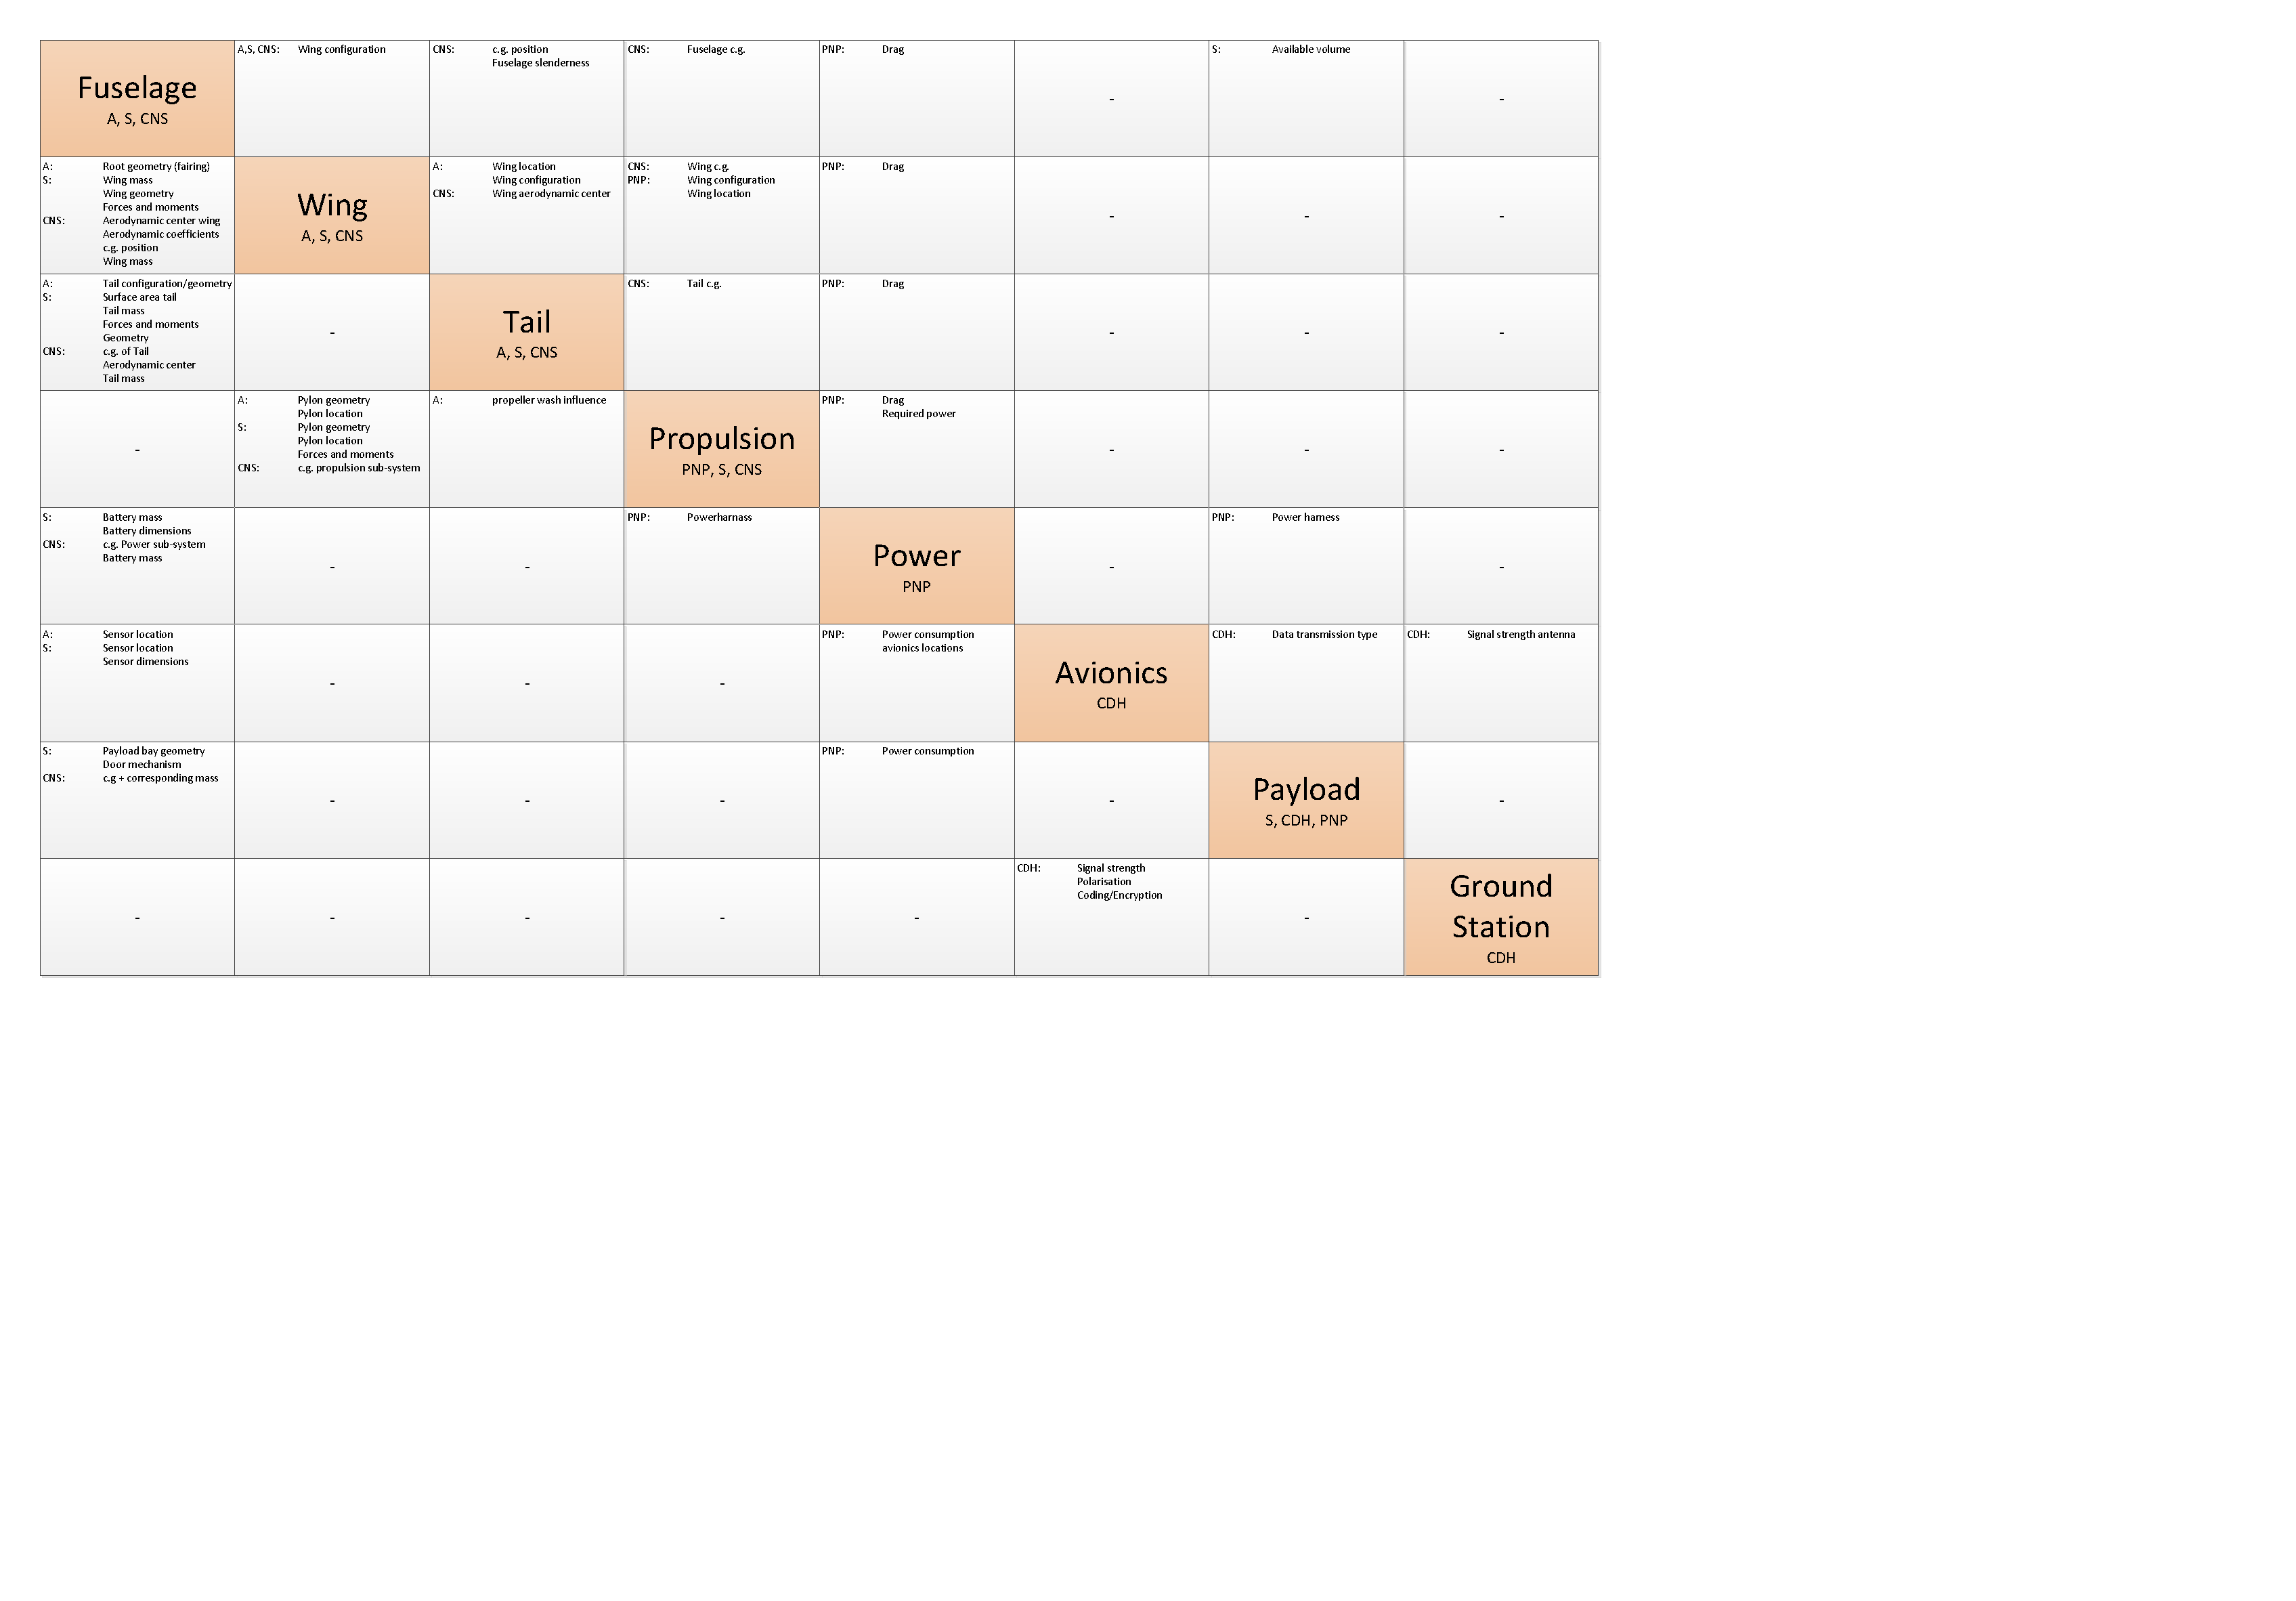
\includepdf[pages=1,fitpaper, scale=0.85,pagecommand={}]{SystemDescription/Figures/N2.pdf}
\label{N2}

\section{Subsystem Requirements}
\label{sec:subs_requ}

The subsystem requirements are presented in this section and are ranked per subsystem. The legend can be found in \autoref{tab:lege}.

\begin{table}[h]
\centering
\caption{Requirements Coding Legend}
\label{tab:lege}
\begin{tabular}{ll}
\toprule
\textbf{Requirement Code} & \textbf{Related to}                       \\\midrule
SUB                       & \textbf{Sub}system                                         \\\hdashline
AV                         & \textbf{Av}ionics                                         \\\hdashline
PR                         & \textbf{Pr}opulsion                                      \\\hdashline
PW                         & \textbf{P}o\textbf{w}er                                 \\\hdashline
W                         & \textbf{W}ing                          \\\hdashline
T                       & \textbf{T}ail       \\\hdashline
F                        & \textbf{F}uselage                      \\\hdashline
P                        & \textbf{P}ayload                      \\\hdashline
GS                        & \textbf{G}round \textbf{S}tation                          \\\bottomrule
\end{tabular}
\end{table}

\subsubsection{Avionics Requirements}
\begin{enumerate}[leftmargin =3.5cm, align=parleft, labelwidth=8em]
    \item[\textbf{SUB-AV-1.1:}] The avionics subsystem shall be able to process flight control and communication data.
    \item[\textbf{SUB-AV-1.2:}] The avionics subsystem shall be insulated to withstand temperatures of -30 to 40 degrees.
    \item[\textbf{SUB-AV-2.1:}] The avionics subsystem shall have a database of restricted areas where it cannot fly.
    \item[\textbf{SUB-AV-2.2:}] The avionics subsystem shall be able to update the restricted areas database.
    \item[\textbf{SUB-AV-2.3:}] The avionics subsystem shall be able to give its geographical position at an accuracy of at least 5 m.
    \item[\textbf{SUB-AV-2.4:}] The avionics subsystem shall be able to determine its distance to the nearest restricted areas.
    \item[\textbf{SUB-AV-2.5:}] The avionics subsystem shall be able to determine its attitude at an accuracy of at least 0.5 degrees per axis.
    %\item[\textbf{SUB-AV-2.6:}] The UAV shall be able to detect weather conditions within [tbd] m.
    \item[\textbf{SUB-AV-2.7:}] The avionics subsystem shall be able to get updates on weather forecasts.
    \item[\textbf{SUB-AV-2.8:}] The avionics subsystem shall be able to return to the base autonomously in case of loss of data link for a period of 10 sec.
    \item[\textbf{SUB-AV-2.10:}] The avionics subsystem shall be able to determine its angular velocity at an accuracy of at least 0.05 deg/sec per axis.
    \item[\textbf{SUB-AV-2.11:}] The avionics subsystem shall be able to determine its angular acceleration at an accuracy of at least 0.01 deg/sec per axis.
    \item[\textbf{SUB-AV-3.1:}] The avionics subsystem shall be able to avoid obstacles.
    \item[\textbf{SUB-AV-3.2:}] The avionics subsystem shall be able to detect all objects within 3 km in front of it.
    \item[\textbf{SUB-AV-3.3:}] The avionics subsystem shall be able to detect the ground when it is within 80 m.
    \item[\textbf{SUB-AV-4.1:}] The avionics subsystem shall be able to fly autonomously.
    \item[\textbf{SUB-AV-4.2:}] The avionics subsystem shall be able to autonomously detect a suitable landing spot.
    \item[\textbf{SUB-AV-4.3:}] The avionics subsystem shall be able to take-off autonomously.
    \item[\textbf{SUB-AV-4.4:}] The avionics subsystem shall be able to land autonomously.
    \item[\textbf{SUB-AV-5.2:}] The avionics subsystem shall automatically descend to 130 m when reaching a height of 150 m.
    \item[\textbf{SUB-AV-6.1:}] The avionics subsystem shall provide a connection to the payload module.
    \item[\textbf{SUB-AV-7.1:}] The avionics subsystem shall make use of a fly-by-wire system.
    \item[\textbf{SUB-AV-8.2:}] The avionics subsystem shall be able to receive inputs from the ground station within a distance of 200 km from the ground station.
    \item[\textbf{SUB-AV-8.3:}] The avionics subsystem shall be albe to transmit data to the ground station within a distance of 200 km from the ground station.
    \item[\textbf{SUB-AV-8.4:}] The data send by the UAV shall be send securely.
    \item[\textbf{SUB-AV-9.1:}] The avionics subsystem shall provide throttle control for motors.
    \item[\textbf{SUB-AV-9.2:}] The avionics subsystem shall control orientation of motors.
\end{enumerate}

\subsubsection{Propulsion Requirements}

\begin{enumerate}[leftmargin =3.5cm, align=parleft, labelwidth=8em]
    %\item[\textbf{SUB-PR-1.1}] The propulsion subsystem shall have a maximum mass of 3.8 kg.
    %\item[\textbf{SUB-PR-1.2}] The propulsion subsystem shall have a maximum cost of 1800 \euro.
    %\item[\textbf{SUB-PR-1.3}] The propulsion subsystem shall require a maximum of 2553 kJ of energy during one mission.
    \item[\textbf{SUB-PR-2.2:}] The propulsion subsystem shall provide thrust in vertical and horizontal flight.
    %\item[\textbf{SUB-PR-2.3:}] The propulsion subsystem shall provide a minimum of 1380 W of power.
    \item[\textbf{SUB-PR-2.4:}] The propulsion subsystem shall provide a minimum thrust of 392 N.
    \item[\textbf{SUB-PR-2.5:}] The propulsion subsystem shall be capable of sustaining a flight velocity of 200 km/h.
    \item[\textbf{SUB-PR-3.4:}] The propulsion subsystem shall be able to provide an angular acceleration of 0.8 $rad/s^{2}$ in roll.
    \item[\textbf{SUB-PR-3.5:}] The propulsion subsystem shall be able to provide an angular pitching acceleration of 0.8 $rad/s^{2}$. 
    \item[\textbf{SUB-PR-3.6:}] The propulsion subsystem shall be able to provide an angular acceleration of 0.1 $rad/s^{2}$ in yaw.
    \item[\textbf{SUB-PR-5.1:}] The propulsion subsystem shall have a maximum noise emission of 68 dB.
\end{enumerate}

\subsubsection{Power Requirements}

\begin{enumerate}[leftmargin =3.5cm, align=parleft, labelwidth=8em]
    \item[\textbf{SUB-PW-1.2:}] The power subsystem shall have a nominal capacity of minimum 1 kWh. 
    \item[\textbf{SUB-PW-1.3:}] The power subsystem shall provide a voltage of 37 V.
    \item[\textbf{SUB-PW-1.4:}] The battery shall be detachable.
\end{enumerate}

\subsubsection{Wing Requirements}

\begin{enumerate}[leftmargin =3.5cm, align=parleft, labelwidth=8em]
    %\item[\textbf{SUB-W-1.1}] The wing subsystem shall have a maximum mass of 4 kg.
    %\item[\textbf{SUB-W-1.2}] The wing shall have a maximum production cost of 900 \euro.
    \item[\textbf{SUB-W-2.1:}] The wing shall provide a minimum lift of 245.25 N in horizontal flight.
    \item[\textbf{SUB-W-2.2:}] The wing shall have a maximum stall velocity of 20 m/s.
    \item[\textbf{SUB-W-2.3:}] The wing tip shall not stall first.
    \item[\textbf{SUB-W-2.4:}] The wing shall have a maximum span of 4.8 meters.
    \item[\textbf{SUB-W-2.5:}] The wing shall have a maximum cantilever ratio of 25.
    \item[\textbf{SUB-W-3.1:}] The wing shall provide sufficient space for its internal components.
    \item[\textbf{SUB-W-3.2:}] The wing shall provide mounting points for the engine pylons. 
    \item[\textbf{SUB-W-3.4:}] The wing shall protect its internal components from dust particles.
    \item[\textbf{SUB-W-3.5:}] The wing shall protect its internal components from precipitation.
    \item[\textbf{SUB-W-3.9:}] The wing shall have a maximum wing tip deflection of 15\% of the wing span.
    \item[\textbf{SUB-W-3.10:}] The wing shall have a maximum wing tip twist angle of $2^{\circ}$.    
    \item[\textbf{SUB-W-3.11:}] The wing shall be designed for a load safety factor of 1.5.
    \item[\textbf{SUB-W-3.14:}] It shall be possible to detach the wing from the fuselage by one person within 2 minutes.
    \item[\textbf{SUB-W-3.16:}] The wing shall not experience aeroelastic flutter at velocities below 220 km/h.
    \item[\textbf{SUB-W-5.6:}] The engine pylons shall not experience aeroelastic flutter at velocities below 220 km/h.
    \item[\textbf{SUB-W-7.2:}] The wing airfoil shall start stalling at the leading edge.
    \item[\textbf{SUB-W-7.3:}] The wing subsystem shall provide an minimal angular roll acceleration of 45 $deg/s^{2}$.   
\end{enumerate}

\subsubsection{Tail Requirements}

\begin{enumerate}[leftmargin =3.5cm, align=parleft, labelwidth=8em]
    \item[\textbf{SUB-T-1.1:}] The tail shall not experience deep stall conditions. 
    \item[\textbf{SUB-T-1.2:}] The tail shall stall after the wing.
    \item[\textbf{SUB-T-2.1:}] The tail shall provide a longitudinal balancing moment for all flight velocities. 
    \item[\textbf{SUB-T-2.2:}] The tail shall be able to provide an angular pitch acceleration of 45 $deg/s^{2}$ in horizontal flight.
    \item[\textbf{SUB-T-2.3:}] The tail shall be able to provide an angular yaw acceleration of 6 $deg/s^{2}$ in horizontal flight.
    \item[\textbf{SUB-T-3.1:}] The tail shall provide sufficient internal space for relevant components.
    \item[\textbf{SUB-T-3.2:}] The tail shall protect internal components from wind.
    \item[\textbf{SUB-T-3.3:}] The tail shall protect internal components from dust. 
    \item[\textbf{SUB-T-3.4:}] The tail shall protect internal components from precipitation.
    \item[\textbf{SUB-T-3.5:}] The tail shall protect internal components from UV radiation.
    \item[\textbf{SUB-T-4.1:}] The tail elevator shall have a maximum deflection angle of 28$^\circ$.
    \item[\textbf{SUB-T-4.2:}] The tail rudder shall have a maximum deflection angle of 25$^\circ$.
    \item[\textbf{SUB-T-5.1:}] The tail shall not contain materials posing a health or environmental threat.
\end{enumerate}

\subsubsection{Fuselage Requirements}

\begin{enumerate}[leftmargin =3.5cm, align=parleft, labelwidth=8em]
    \item[\textbf{SUB-F-1.1:}] The fuselage shall contain at least 1 kg of permanent batteries. 
    \item[\textbf{SUB-F-1.2:}] The fuselage shall provide mounting points for internal and external UAV components.
    \item[\textbf{SUB-F-2.1:}] The fuselage shall protect internal components from wind.
    \item[\textbf{SUB-F-2.2:}] The fuselage shall protect internal components from dust.
    \item[\textbf{SUB-F-2.3:}] The fuselage shall protect internal components from precipitation.
    \item[\textbf{SUB-F-2.4:}] The fuselage shall protect internal component from UV radiation.
    \item[\textbf{SUB-F-3.1:}] The fuselage shall not fail when a belly landing of 4 m/s is performed.
    \item[\textbf{SUB-F-4.1:}] The fuselage shall not contain materials that pose health or environmental threats.
\end{enumerate}

\subsubsection{Payload Requirements}

\begin{enumerate}[leftmargin =3.5cm, align=parleft, labelwidth=8em]
    \item[\textbf{SUB-P-2.1:}] The payload subsystem shall have a two-way power link with the fuselage.
    \item[\textbf{SUB-P-2.2:}] The payload subsystem power link shall be rated for a minimum of 50 W.
    \item[\textbf{SUB-P-3.3:}] The payload subsystem shall provide mounting points for the payload (including additional batteries).
    \item[\textbf{SUB-P-3.4:}] The payload subsystem shall allow for payload release during flight.
\end{enumerate}

\subsubsection{Ground Station Requirements}

\begin{enumerate}[leftmargin =3.5cm, align=parleft, labelwidth=8em]
    \item[\textbf{SUB-GS-2.1:}] The ground station shall be able to process all data received by the UAV. 
    \item[\textbf{SUB-GS-3.2:}] The ground station battery shall enable at least two hours of consequal operating.
    \item[\textbf{SUB-GS-4.1:}] The ground station shall transmit inputs to the UAV within a distance of 200 km.
    \item[\textbf{SUB-GS-4.2:}] The ground station shall be able to receive data from the UAV within a distance of 200 km.
    \item[\textbf{SUB-GS-4.3:}] The ground station shall send data towards the UAV securely.
    \item[\textbf{SUB-GS-4.7:}] The ground station shall be able to communicate with the drone in stormy weather conditions.
    \item[\textbf{SUB-GS-5.1:}] The ground station casing shall fit within 100x50x30 cm.
    \item[\textbf{SUB-GS-5.2:}] The ground station shall weigh at most 7.5 kg.
    \item[\textbf{SUB-GS-5.3:}] All ground system components shall be easily replaceable.
    \item[\textbf{SUB-GS-6.2:}] The ground station shall have a display that can show mission specific information.
    \item[\textbf{SUB-GS-6.3:}] The ground station shall be able to control the UAV.
    \item[\textbf{SUB-GS-6.4:}] The ground station shall be able to make the UAV drop the payload.
    \item[\textbf{SUB-GS-7.1:}] The ground station shall displaye a warning when exceeding a height of 140 m from the ground.
    \item[\textbf{SUB-GS-7.2:}] The ground station shall display a warning when approaching a restricted area.
\end{enumerate}




\section{Budgets \& Contingencies}
\label{sec:budg_cont}
To ensure that the departments do not exceed any limits during the designing, some budgets have been made. On top of the budgets a contingency is added. There are two budgets: the mass budget and the cost budget. The ground control is not considered in the budgets as it is seen as a separate system. The final budgets and contingencies for mass and cost can be found in \autoref{tab:massbudget}. 

\begin{table}[H]
    \centering
    \caption{Mass and Cost Budget for the Aircraft}
    \label{tab:massbudget}
    \begin{tabular}{ccccc} \toprule
    
    
    
    \bfseries Subsystem     & \bfseries Mass Budget &\bfseries Contingency & \bfseries Cost Budget &\bfseries  Contingency \\ \midrule
    Power     & 8.0 kg & 5\% & 800 EUR& 5\%  \\
    Propulsion & 4.0 kg & 5\% & 2200 EUR& 10\% \\
    Avionics & 1.0 kg & 5\% & 2200 EUR & 10\% \\
    Wing & 3.5 kg & 10\% & 800 EUR& 10\% \\
    Tail & 1.5 kg & 10\% & 400 EUR& 10\% \\
    Fuselage & 2.5 kg & 10\% & 800 EUR& 10\% \\
    Payload & 4.5 kg & 5\% & 300 EUR& 5\% \\ \bottomrule
    \end{tabular}
\end{table}


\paragraph{Mass Budget}
The mass budget has been estimated by comparing it to a similar UAV, the Avy One\footnote{\url{avy.eu}, Accessed on 21-06-2017}. This aircraft has a Manufacturing Empty Weight (MEW) of 13 kg, meaning that if this design has a maximum mass of 25 kg, 12 kg are allotted to the battery and payload. The other 13 kg are destined for the structure of the aircraft\footnote{Private Contact Avy, 22-05-2017}. The mass budget can be seen in \autoref{tab:massbudget}. To have an allowable margin of freedom, contingencies are put in place for each subsystem. The percentage of the contingency varies with the certainty of the mass budget. The contingency should decrease over time as the project progresses, and the mass prediction becomes more precision.

\paragraph{Cost Budget}
Analysing the cost budget has been done in a similar fashion as the mass budget. Contact has been established between Atmos, a company which produces the Marlyn\footnote{\url{http://www.atmosuav.com/}, Accessed on 22-06-2017}, a UAV similar to the Winged Quadcopter. This company provided information about how much percent of the cost their subsystems take up. Before budgeting the cost of each subsystem, the choice has been made to separate the cost of materials from the cost of manufacturing. The assumption has been made that 75\% of the costs are attributed to manufacturing. This leaves 7.5k EUR for materials of the subsystems. The percentage of cost for the Marlyn can be seen in \autoref{tab:costperc}\footnote{Private Contact Atmos, 08-06-2017}.

\begin{table}[H]
    \centering
    \caption{Percentage of Cost for the Atmos UAV}
    \begin{tabular}{rl} \toprule
    \bfseries Subsystem &\bfseries Percentage of Cost \\\midrule
    Power \& Propulsion     &  20\% \\
    Payload     & 10\% \\
    Avionics & 20\% \\
    Wing, Tail \& Fuselage & 40\% \\
    Contingency & 10\% \\\bottomrule
    \end{tabular}

    \label{tab:costperc}
\end{table}

With these values, it is possible to devise the cost budget. The Atmos UAV has its cameras added to the payload cost, which this design does not have. This means that a part of their payload cost can be neglected. Atmos has said that the avionics will take up a larger percentage of the total cost for this design since they have designed and built parts of the avionics by themselves. The wing and fuselage turn out to cost the same amount, while the tail costs half of the wing \cite{costbreakdown}. 

Using the preliminary energy calculation from the midterm report \cite{midterm}, the cost of the power subsystem is estimated to be 800 EUR. The rest of the cost is attributed to the propulsion subsystem, which turns out to be close to 20\% as estimated by Atmos. The final cost budget can be seen in \autoref{tab:massbudget}.

